%%%%%%%%%%%%%%%%%%%%%%%%%%%%%%%%%%%%%%%%%
% Beamer Presentation
% LaTeX Template
% Version 1.0 (10/11/12)
%
% This template has been downloaded from:
% http://www.LaTeXTemplates.com
%
% License:
% CC BY-NC-SA 3.0 (http://creativecommons.org/licenses/by-nc-sa/3.0/)
%
%%%%%%%%%%%%%%%%%%%%%%%%%%%%%%%%%%%%%%%%%

%----------------------------------------------------------------------------------------
%	PACKAGES AND THEMES
%----------------------------------------------------------------------------------------

\documentclass[10pt]{beamer}

\mode<presentation> {

% The Beamer class comes with a number of default slide themes
% which change the colors and layouts of slides. Below this is a list
% of all the themes, uncomment each in turn to see what they look like.

%\usetheme{default}
%\usetheme{AnnArbor}
%\usetheme{Antibes}
%\usetheme{Bergen}
%\usetheme{Berkeley}
%\usetheme{Berlin}
%\usetheme{Boadilla}
%\usetheme{CambridgeUS}
%\usetheme{Copenhagen}
%\usetheme{Darmstadt}
%\usetheme{Dresden}
%\usetheme{Frankfurt}
%\usetheme{Goettingen}
%\usetheme{Hannover}
%\usetheme{Ilmenau}
%\usetheme{JuanLesPins}
%\usetheme{Luebeck}
%\usetheme{Madrid}
%\usetheme{Malmoe}
%\usetheme{Marburg}
%\usetheme{Montpellier}
%\usetheme{PaloAlto}
%\usetheme{Pittsburgh}
\usetheme{Rochester}
%\usetheme{Singapore}
%\usetheme{Szeged}
%\usetheme{Warsaw}

% As well as themes, the Beamer class has a number of color themes
% for any slide theme. Uncomment each of these in turn to see how it
% changes the colors of your current slide theme.

%\usecolortheme{albatross}
%\usecolortheme{beaver}
%\usecolortheme{beetle}
\usecolortheme{crane}
%\usecolortheme{dolphin}
%\usecolortheme{dove}
%\usecolortheme{fly}
%\usecolortheme{lily}
%\usecolortheme{orchid}
%\usecolortheme{rose}
%\usecolortheme{seagull}
%\usecolortheme{seahorse}
%\usecolortheme{whale}
%\usecolortheme{wolverine}

%\setbeamertemplate{footline} % To remove the footer line in all slides uncomment this line
%\setbeamertemplate{footline}[page number] % To replace the footer line in all slides with a simple slide count uncomment this line

%\setbeamertemplate{navigation symbols}{} % To remove the navigation symbols from the bottom of all slides uncomment this line
}

\usepackage{graphicx} % Allows including images
\usepackage{booktabs} % Allows the use of \toprule, \midrule and \bottomrule in tables
\usepackage{listings}

%----------------------------------------------------------------------------------------
%	TITLE PAGE
%----------------------------------------------------------------------------------------

\title[Improved Execution Migration]{Improved Execution Migration} % The short title appears at the bottom of every slide, the full title is only on the title page

\author{Meet Udeshi, Nirmal Boran} % Your name
\institute[IIT Bombay] % Your institution as it will appear on the bottom of every slide, may be shorthand to save space
{
IIT Bombay\\ % Your institution for the title page
}
\date{\today} % Date, can be changed to a custom date

\begin{document}

\begin{frame}
\titlepage % Print the title page as the first slide
\end{frame}

%\begin{frame}
%\frametitle{} % Table of contents slide, comment this block out to remove it
%\tableofcontents % Throughout your presentation, if you choose to use \section{} and \subsection{} commands, these will automatically be printed on this slide as an overview of your presentation
%\end{frame}

%----------------------------------------------------------------------------------------
%	PRESENTATION SLIDES
%----------------------------------------------------------------------------------------
% : Simultaneous transformation, frame-wise transformation, loop migration, live variable optimisation
%------------------------------------------------
\section{Execution Migration Introduction} % Sections can be created in order to organize your presentation into discrete blocks, all sections and subsections are automatically printed in the table of contents as an overview of the talk
%------------------------------------------------

%\subsection{Subsection Example} % A subsection can be created just before a set of slides with a common theme to further break down your presentation into chunks

\begin{frame}
\frametitle{Introduction}
\begin{itemize}
\item Venkat et al\footnote{\tiny{A.Venkat, D.Tullsen - Harnessing ISA Diversity: Design of a Heterogeneous-ISA Chip Multiprocessor}}
    show energy efficiency and performance gain by Heterogenous ISA CMPs.
\item DeVuyst et al\footnote{\tiny{M.DeVuyst et al - Execution Migration in a Heterogeneous-ISA Chip Multiprocessor}} explore cost-effective migration strategies.
\begin{itemize}
    \item Global variables kept common during compile-time.
    \item Heap memory only touched by \textit{malloc} function, same implementation used.
    \item Keep functions at same virtual address for same pointers.
    \item Stack frame size and local variable location maintained same at compile time by using padding.
    \item \textbf{Dynamic modification:} Hard-coded stack offset in instructions, function arguments, stack object pointers.
\end{itemize}
\item DeVuyst et al look at only function calls as potential migration points, and suggest using binary translation for immediate shift until a migration point is reached.
\end{itemize}
\end{frame}

\section{Implementation and challenges}
\begin{frame}
\frametitle{Implementation and Challenges}
    \begin{itemize}
    \item LLVM compiler (\texttt{clang} and \texttt{llc}) for analysis of function stack-frames for stack transformation.
    \item Mapping variables in C code, or even LLVM-IR to stack slots is difficult when using \texttt{-O1} or higher. Resort to compiling with \texttt{-O0}.
    \item Callee-saved spilled register mapping depends heavily on live variables at call-site.
    \item Pointer values in callee have to be changed when caller stack is transformed. Mapping pointer to variable is difficult, because a function can be passed pointers by multiple functions.
    \end{itemize}
\end{frame}

%------------------------------------------------

\section{Suggested Improvements}

\subsection{Simultaneous transformation}

\begin{frame}
\frametitle{Simultaneous transformation}
Only last frame on the stack (current function) is currently in use.
Start transformation of other frames simultaneously on other processor before migration point is reached.

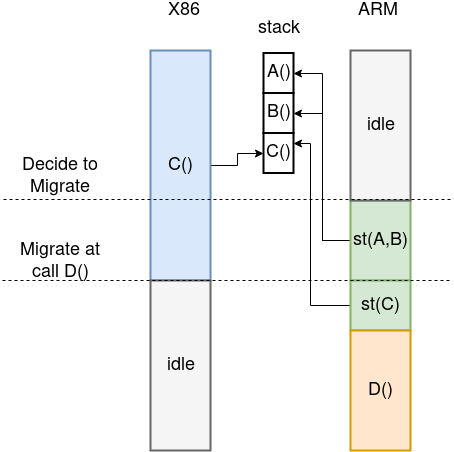
\includegraphics[width=0.55\textwidth]{simul_trans}
\end{frame}

\begin{frame}
\frametitle{Simultaneous transformation}

\textbf{Problem:}
\begin{itemize}
\item Stack transformer implementation given in paper requires two-pass transformation
\item First pass is frame-wise and can be handled in parallel.
\item Second pass fixes corner-case of pointers and does register mapping in between ISA based on live variables.
\end{itemize}
\end{frame}


%\subsection{Migration at loop branches}

%\begin{frame}
%\frametitle{Migration at loop branches}
%\begin{itemize}
%\item As seen in graphic, some programs spend a lot of time inside loops.
%\item Loop branches (jmp instruction to loop start label) will be present in both ISA.
%\item Migration at this point will be able to harness efficiency for further loop iterations.
%\item Binary translation not necessary because migration points will be much more frequent.
%\end{itemize}

%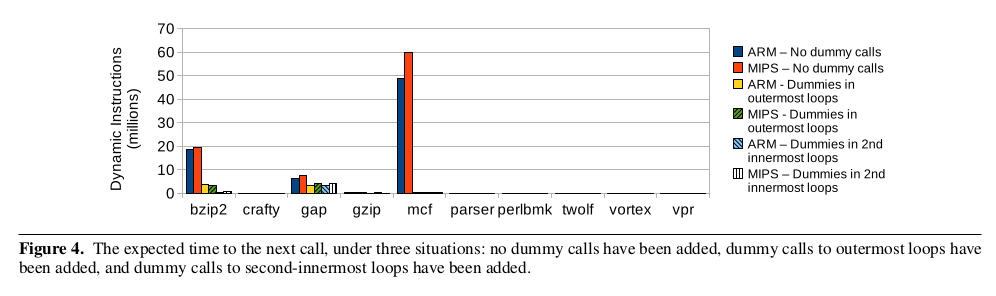
\includegraphics[width=0.95\textwidth]{migration_freq}
%\end{frame}


\subsection{Single frame transformation}

\begin{frame}
\frametitle{Single frame transformation}
Only transform the stack frame of current function.

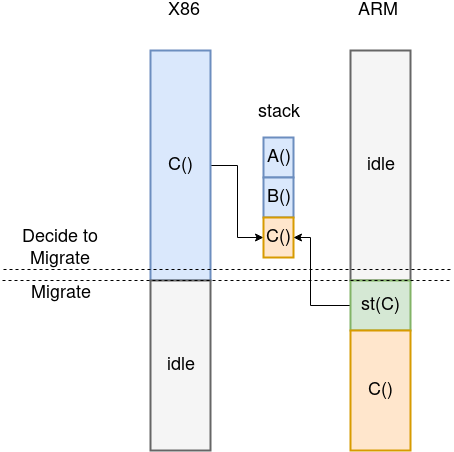
\includegraphics[width=0.55\textwidth]{singleframe_trans}
\end{frame}

\begin{frame}
\frametitle{Single frame transformation}
When returning to previous function, decide whether to migrate to current processor or switch to previous processor

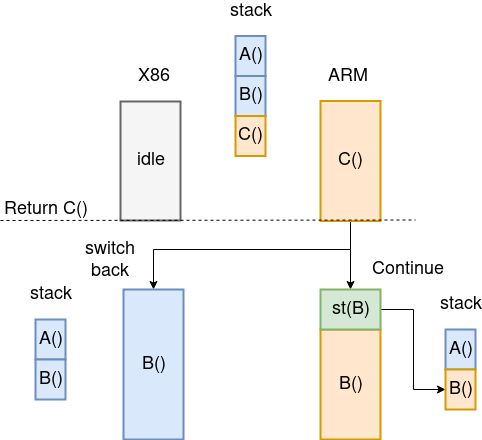
\includegraphics[width=0.55\textwidth]{singleframe_return}
\end{frame}



\begin{frame}
\frametitle{Single frame transformation}

\textbf{Advantages:}
\begin{itemize}
\item Pointer problem solved. Pointer value not changed because previous stack not modified.
\end{itemize}
\textbf{Problems:}
\begin{itemize}
\item Live variables in registers would have to be moved twice, or added to the stack.
\item Migration on function return, would require live variable analysis.
\end{itemize}
\end{frame}

\section{Transformation pseudo-code}
\begin{frame}[fragile]
\frametitle{Transformation pseudo-code}

\textbf{Function:} \verb|BZ2_bzDecompressInit(bz_stream*, int, int)|

\begin{columns}

\begin{column}{0.4\textwidth}

\begin{tabular}{lccc}
\textbf{Slot} & \textbf{size} & \textbf{align} & \textbf{location} \\
\hline
x86: & & & \\
\hline
  \textit{fi.0} & 4 & 4 & [SP-28] \\
  \textit{fi.1} & 8 & 8 & [SP-24] \\
  \textit{fi.2} & 4 & 4 & [SP-36] \\
  \textit{fi.3} & 4 & 4 & [SP-32] \\
  \textit{fi.4} & 8 & 8 & [SP-16] \\
\hline
ARM: & & & \\
\hline
  \textit{fi.0} & 4 & 4 & [SP-20] \\
  \textit{fi.1} & 8 & 8 & [SP-32] \\
  \textit{fi.2} & 4 & 4 & [SP-36] \\
  \textit{fi.3} & 4 & 4 & [SP-40] \\
  \textit{fi.4} & 8 & 8 & [SP-48] \\
\end{tabular}
\end{column}

\begin{column}{0.5\textwidth}
\begin{lstlisting}
tmp1 = frame[loc[1]]
frame[loc[1]] = frame[loc[0]]

for i=2..len(loc):
    tmp2 = frame[loc[i]]
    frame[loc[i]] = tmp1
    tmp1 = tmp2
\end{lstlisting}

\end{column}
\end{columns}

\end{frame}

\begin{frame}[fragile]
\frametitle{Pointer Analysis}
\begin{lstlisting}
define @functionA
  %2 = alloca i32
  %3 = alloca i64
    .
    .
  %51 = load i64, %3 i64*
  %52 = call @functionB(%51 i64, %2 i32*)
\end{lstlisting}

In LLVM-IR, alloca instruction return the pointer to stack variable, which is kept in the first few SSA variables of the function. We can determine these SSA variables by looking for alloca instructions. Thus, use of these variables in function calls would mean a pointer to the stack is being passed to child function.

Only 5 such cases were found in the entire bzip2 package.
\end{frame}

\subsection{Simulation and Results}

\begin{frame}
\frametitle{Simulation method}

    \begin{itemize}
        \item Migration between X86\_64 and Aarch64 ISA
        \item Implemented migration code in \texttt{C} as \texttt{migrate()} function
        \item \texttt{migrate()} call is inserted at end of (almost) every function in codebase
        \item Used \texttt{gem5} to calculate time of execution for \texttt{migrate()}
    \end{itemize}
\end{frame}

\begin{frame}
\frametitle{Simulation Results}

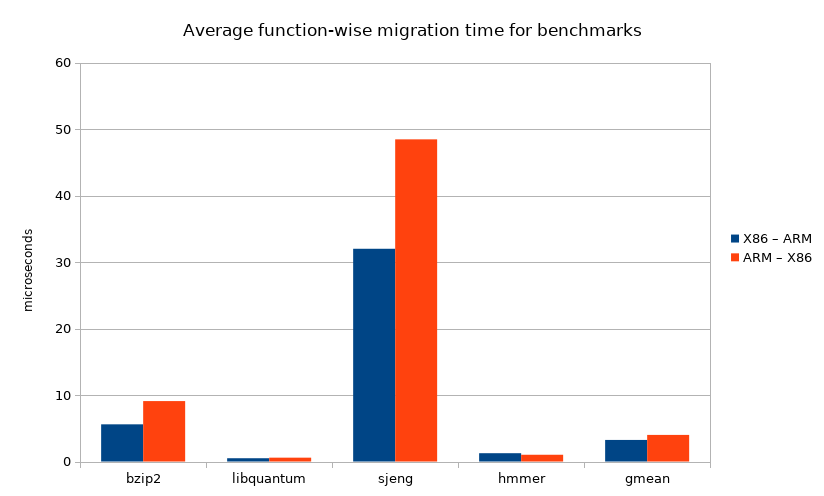
\includegraphics[width=0.49\textwidth]{our-plot}
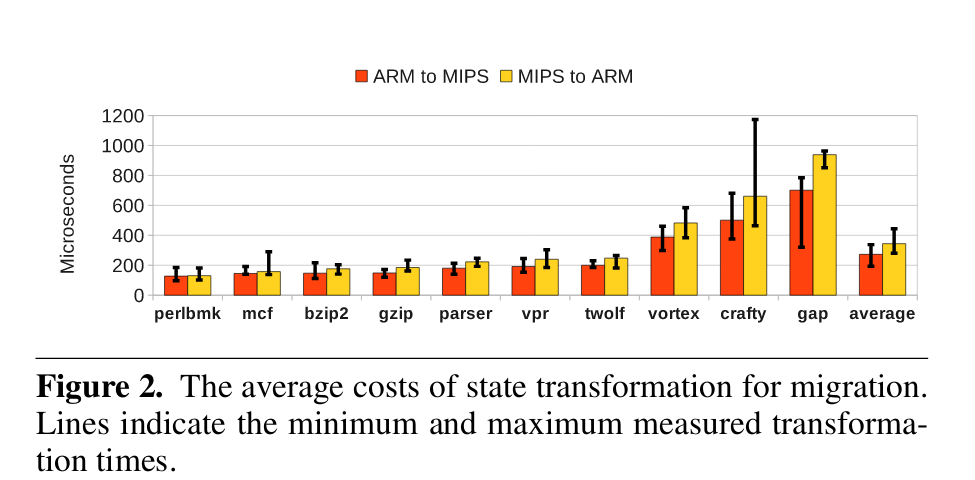
\includegraphics[width=0.49\textwidth]{tullsen-plot}

\end{frame}

%%\begin{frame}
%\frametitle{Future work}
%\begin{itemize}
%\item Generating data for every call-site, if we take migration to only happen at function calls. ($\sim 220$ call-sites for bzip2 package)
%\item Data for Live-variables and pointers of stack objects can be determined at compile time.
%\item At runtime, determine every call site based on return addresses.
%\item Use compile-time data to finish stack transformation.
%\end{itemize}
%\end{frame}

%\subsection{Live variables}

%\begin{frame}
%\frametitle{Live variables}
%\begin{itemize}
%\item At some execution point in the function, there will be live and dead variables on the stack.
%\item Optimisation to stack transformer to ignore dead variables can reduce migration cost.
%\item Compiler will assist in keeping track of live+dead variables.
%\end{itemize}

%\end{frame}

%------------------------------------------------

\begin{frame}
\Huge{\centerline{The End}}
\end{frame}

%----------------------------------------------------------------------------------------

\end{document}
